\chapter{Preimage Attack on 2-Rounds of \KECCAK{}${[r:=800-384, c:=384]}$}

In this chapter we present a new preimage attack on $2$ rounds of \KECCAK{}$[r:=800-384, c:=384]$. We will show that the preimage can be found in $O(2^{44})$ time and $O(2^{42})$ memory for $2$ rounds of round-reduced \KECCAK{}$[r:=800-384, c:=384]$. It is a practical attack, and also it is an improvement over the existing best-known attack, for $2$ rounds of \KECCAK{}$[r:=800-384, c:=384]$, which has a time complexity of $O(2^{64})$~\cite{guo2016linear}.

\section{Description of the Attack}
\label{2rkeccak800attack}
The \KECCAK{}$[r:=800-384, c:=384]$ has rate $r = 800-384 = 416$, capacity $c = 384$ and outputs a hash of $192$ bits, which is represented by the first $6$ lanes ($lanesize = 32$ bits) in the state obtained at the end of the squeezing phase. Figure~\ref{initial_sq} represents the hash state. In the hash state except the first $6$ lanes, we don't care about other lanes i.e. remaining $19$ lanes. We are interested in finding a preimage for which $6$ lanes of corresponding state matches. We will call this state as \emph{final state}.
%------------------------------------------------
\begin{figure}[ht]
\begin{center}
\begin{tikzpicture}[ampersand replacement=\&]
\matrix (sm1) [matrix of nodes,
nodes={inner sep=5pt,text width=0.5cm,align=center,minimum height=.5cm, draw,text height=1em,text depth=.2em}
]{
    $\star$ \& $\star$\& $\star$ \& $\star$ \& $\star$\\
    $\star$ \& $\star$\& $\star$ \& $\star$ \& $\star$\\
    $\star$ \& $\star$\& $\star$ \& $\star$ \& $\star$\\
    $h_5$ \& $\star$\& $\star$ \& $\star$ \& $\star$\\
    $h_0$ \& $h_1$\& $h_2$ \& $h_3$ \& $h_4$\\
};
\node[] at (-1.7,-2.5) { 0 };
\node[] at (-0.85,-2.5) { 1 };
\node[] at (0.0,-2.5) { 2 };
\node[] at (0.9,-2.5) { 3 };
\node[] at (1.8,-2.5) { 4 };
\draw[thick,->] (-1.5, -3.2) -- node [above] {$x$} (0.0, -3.2);
\node[] at (-2.5,-1.5) { 0 };
\node[] at (-2.5,-0.75) { 1 };
\node[] at (-2.5,0.0) { 2 };
\node[] at (-2.5,0.8) { 3 };
\node[] at (-2.5,1.5) { 4 };
\draw[thick,->] (-3, -0.7) --  (-3, 0.8);
\node[] at (-3.3, 0) {$y$};
\end{tikzpicture}
\end{center}
\caption{The Final Hash State for \KECCAK{}$[r:=800-384, c:=384]$ \label{initial_sq}}
\end{figure}
%------------------------------------------------
In this attack, we can ignore the {$\iota$} step mapping without the loss of generality, as it does not affect the procedure of the attack. However it should be taken into account while implementing the attack.

We further note that the initial state, which is fed to \KECCAK-$f$ function, is the first message block which is represented by $25-2\cdot 6$ i.e., $13$ lanes. The remaining $12$ lanes are initially set to $0$. Pictorially, this state is represented by the diagram in the Figure~\ref{initial_state}. We call this state \emph{initial state}.
Our aim is to find the values of $a_0, a_1, a_2$, $b_0, b_1, b_2$, $c_0, c_1, c_2$, $d_0, d_1$ and $e_0, e_1$ variables in the initial state which lead to a final state having first six lanes as $h_0,\;h_1,\;h_2,\;h_3,\;h_4$ and $h_5$. 

We follow the basic idea of the attack, as given in the paper~\cite{naya2011practical}.
We start the attack by setting variables in the initial state which ensures zero column parity. 
This is done by imposing the following restrictions.
\begin{align}\nonumber
a_2 &= a_0 \oplus a_1,\quad b_2 = b_0 \oplus b_1, \quad c_2 = c_0 \oplus c_1\\ \label{cond_state1}
d_1 & = 0,\quad d_0 = 0\;\;\text{ and }\;\; e_1 = e_0. 
\end{align}

\begin{figure}
\begin{center}
\begin{tikzpicture}[ampersand replacement=\&]
\matrix (sm1) [matrix of nodes,
nodes={inner sep=5pt,text width=0.5cm,align=center,minimum height=.5cm, draw,text height=1em,text depth=.2em}
]{
    $0$ \& $0$\& $0$ \& $0$ \& $0$\\
    $0$ \& $0$\& $0$ \& $0$ \& $0$\\
    $a_1$ \& $b_1$\& $c_2$ \& $0$ \& $0$\\
    $a_2$ \& $b_2$\& $c_1$ \& $d_1$ \& $e_1$\\
    $a_0$ \& $b_0$\& $c_0$ \& $d_0$ \& $e_0$\\
};
\end{tikzpicture}
\end{center}
\caption{Setting of Initial State in the Attack\label{initial_state}}
\end{figure}
%--------------------------------------------------------

\begin{figure}[H]
    \centering
    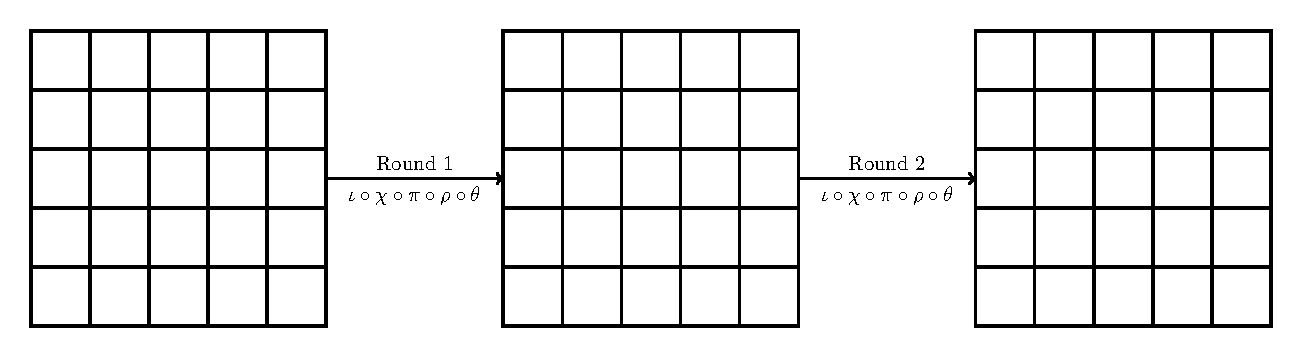
\includegraphics[scale=0.7]{keccak2Rstate.pdf}
    \caption{Two round of \KECCAK$[r:=800-384, c:=384]$}
    \label{two_rnd}
\end{figure}

This type of assignment to the initial state will make the {$\theta$} step mapping, an identity mapping. Even though we have put some restrictions to the initial state, we still find the input space of \KECCAK{}$[r:=800-384, c:=384]$ (with $1$ message block) large enough to ensure first $6$ lanes of output state, the given hash value. We explain the details of the analysis below. 

Note that the output of attack is an assignment to the variables $a_0, a_1, a_2$, $b_0, b_1, b_2$, $c_0, c_1, c_2$, $d_0, d_1$ and $e_0, e_1$, which on applying $2$ rounds of \KECCAK-$f$ gives the target hash value. Recall that we are mounting an attack on the $2$ rounds of \KECCAK{}$[r:=800-384, c:=384]$ (see the diagram in Figure~\ref{two_rnd}).

%\begin{figure}
%\begin{center}
%\begin{tikzpicture}[scale=1.2]
%\node(A1)[]{\grd};
%\node(A2)[right=1.0cm of A1]{\grd};
%\node(A3)[right=1.0cm of A2]{\grd};
%\draw [very thick, ->,] (A1) -- node[above]{{\tt Round$\,1$}} 
%node[below]{$\theta,\rho,\pi,\chi,\iota$} (A2);
%\draw [very thick, ->,] (A2) -- node[above]{{\tt Round$\,2$}} node[below]{$\theta,\rho,\pi,\chi,\iota$}(A3);
%\node [below=0.0cm of A1, xshift=-0.5cm]{Intial State};
%\node [below=0.0cm of A3, xshift=-0.5cm]{Final State};
%\node [below=0.0cm of A2, xshift=-0.5cm]{Intermediate State};
%\end{tikzpicture}
%\caption{Two round of \KECCAK{}$[r:=800-384, c:=384]$\label{two_rnd}}
%\end{center}
%\end{figure}
%
%
The overall attack is summarized in the  diagram given in the Figure~\ref{atk}. 
%
\begin{figure}[!t]
\begin{center}
\resizebox{\textwidth}{!}{%
\begin{tikzpicture}[ampersand replacement=\&, scale=0.5]
\matrix (am1) [matrix of nodes,nodes in empty cells,
nodes={inner sep=5pt,text width=1.0cm,align=center,minimum height=1.0cm, draw,text height=1em,text depth=.2em},
myrow/.list={(1,white),(2,white),(4,gray!30),(5,gray!30)},
mycell/.list={(3,1,gray!30),(3,2,gray!30),(3,3,gray!30),(3,4,white),(3,5,white)}]    
{
    $0$ \& $0$\& $0$ \& $0$ \& $0$\\
    $0$ \& $0$\& $0$ \& $0$ \& $0$\\
    $a_1$ \& $b_1$\& $c_2$ \& $0$ \& $0$\\
    $a_2$ \& $b_2$\& $c_1$ \& $d_1$ \& $e_1$\\
    $a_0$ \& $b_0$\& $c_0$ \& $d_0$ \& $e_0$\\
};
\matrix (am2) [right=1.5 cm of am1,matrix of nodes,nodes in empty cells,
nodes={inner sep=5pt,text width=1.0cm,align=center,minimum height=1.0cm, draw,text height=1em,text depth=.2em},
mycolumn/.list={(1,gray!30),(2,gray!30),(4,white),(5,white)},
mycell/.list={(1,3,white),(3,3,white),(2,3,gray!30),(4,3,gray!30),(5,3,gray!30)}
]    
{
    $c_0(30)$ \& $d_1(23)$ \& $0$         \& $0$ \& $0$\\
    $e_0(27)$ \& $a_2(4)$ \& $b_1(10)$ \& $0$ \& $0$\\
    $b_0(1)$  \& $c_1(6)$  \& $0$         \& $0$ \& $0$\\
    $d_0(28)$ \& $e_1(20)$ \& $a_1(3)$  \& $0$ \& $0$\\
    $a_0(0)$  \& $b_2(12)$ \& $c_2(11)$ \& $0$ \& $0$\\
};

\matrix (am3) [below=1.5 cm of am2,matrix of nodes,nodes in empty cells,
nodes={inner sep=5pt,text width=1.0cm,align=center,minimum height=1.0cm, draw,text height=1em,text depth=.2em, fill=gray!10},
mycell/.list={(5,1,gray!50),(4,2,gray!50),(3,3,gray!50),(2,4,gray!50),(1,5,gray!50),(5,4,gray!50),(4,5,gray!50)}
]    
{
        \&      \&       \&      \& $h_4^\prime(18)$\\
        \&      \&       \&$h_3^\prime(11)$ \&         \\
        \&      \& $h_2^\prime(21)$\&      \&         \\
        \&$h_1^\prime(20)$ \&       \&      \& $1$        \\
  $h_0^\prime(0)$ \&         \&      \& $h_5^\prime(4)$     \&         \\
};
\matrix (am4) [left=1.50 cm of am3,matrix of nodes,nodes in empty cells,
nodes={inner sep=5pt,text width=1.0cm,align=center,minimum height=1.0cm, draw,text height=1em,text depth=.2em, fill=gray!10},
mycell/.list={(5,1,gray!50),(5,2,gray!50),(5,3,gray!50),(5,4,gray!50),(5,5,gray!50),(4,1,gray!50)}
]    
{
    \&  \&   \&  \& \\
    \&  \&   \&  \& \\
    \&  \&   \&  \& \\
    $h_5$ \&  \&   \&  \& \\
    $h_0$ \& $h_1$\& $h_2$ \& $h_3$ \& $h_4$\\
};

\node[ below=0.2cm of am1-5-3]{\bf State~1};
\node[ below=0.2cm of am2-5-4]{\bf State~2};
\node[ below=0.2cm of am3-5-3]{\bf State~3};
\node[ below=0.2cm of am4-5-3]{\bf State~4};
\draw[->, very thick] (am1)-- node[above]{$\theta, \pi,\rho$} (am2);
\draw[->, very thick] (am2)-- node[left]{$\chi, \iota,\theta$} (am3);
\draw[->, very thick] (am4)-- node[above, pos=0.4]{$\iota^{-1},\chi^{-1}$} node[below, pos=0.6]{$ \pi^{-1},\rho^{-1}$} (am3);
\end{tikzpicture}
}
\caption{Diagram for $2$-round preimage attack on \Keccak-$384$ \label{atk}}
\end{center}
\end{figure}
%-------------------------------------
The State~$2$, in the Figure~\ref{atk}, represents the state after $\pi \circ \rho \circ \theta$ is applied to the State~$1$. 
The $\theta$-mapping becomes identity due to the condition (Equation~\ref{cond_state1}) imposed on the initial state. The $\rho$ and $\pi$ mappings are, nevertheless, linear.

We are given with a hash value which is represented by first $6$ lanes in the State~$4$ [Figure~\ref{atk}]. It represents the final state ({\tt Round}~2) of \KECCAK{}$[r:=800-384, c:=384]$. The state can be inverted by applying $\chi^{-1} \circ \iota^{-1}$ mapping. The $\iota^{-1}$ is trivial and $\chi^{-1}$ can be computed using the Observations~\ref{ob1} and~\ref{ob2}. The first $7$ lanes of the output is $\{h_0',h_1',h_2',h_3',h_4',h_5',h_6',1\}$. We do not care about the remaining  lanes. 
Then the mappings $\pi^{-1}$ and $\rho^{-1}$ are applied, which are very easy to compute, to get the State~$3$ [Figure~\ref{atk}]. 

Note that, at this point, the blank lanes in the State~$3$, of the Figure~\ref{atk}, could take any random value and this does not have any effect on the target hash value.

The number shown in round brackets along with the variable, in the State~$2$ and State~$3$ [Figure~\ref{atk}], is due to rotation by $\rho$ step mapping in lanes.
On applying $\theta \circ \iota \circ \chi$, operation on the State~$2$, the output should match with the values of the corresponding bits in State~$3$ [Figure~\ref{atk}], then only we can verify and claim that the values of the variables are a preimage for the hash value taken. In the State~$3$, there are $7$ lanes whose values are fixed. 
This will impose a total of $7\times 32$ conditions on the variables we have set in the initial state. As mentioned earlier, we have also set $6$ conditions (see the Equation~\ref{cond_state1}) on the initial state variable and this will further add $7 \times 32$ conditions. So there are in total $13\times 32$ conditions. Since the number of variables and the number of conditions is equal, we can expect to find one solution and it is indeed the case. In the rest of this section, we provide an algorithm to get the preimage for the given hash of  \KECCAK{}$[r:=800-384, c:=384]$. Our method is based on the technique proposed by Naya-Plasencia \etal in the paper~\cite{naya2011practical}.

We aim to find the assignment of bits to the initial state which leads to a target hash value. We proceed as follows. We start with all possible assignments in the groups successive $3$ slices. Using the constraints (transformation from State~2 to State~3 [Figure~\ref{atk}]), we discard some of the assignments, and store the remaining ones, out of which at least one would be a part of the solution. This is done for every $3$-slice from the first $48$ slices. The next step is to merge the two successive $3$-slices. Again we do discard certain choices of assignments and keep the remaining ones. This process is continued to fix a set of good assignments to the $6$-slices, $12$-slices, $16$-slices and $24$-slices groups. In the last, after combining all the assignments we are left with a unique assignment, which is the required preimage. We explain the details in the Section~\ref{sec:partial_sol} below. 

\section{Finding Partial Solutions\label{sec:partial_sol}}
We focus on the two intermediate states of the attack i.e., the State~2 and the State~3 (see the Figure~\ref{atk_partial} below). Note that, since $d_0$ and $d_1$ are set to $0$ in the beginning, we are now left with $11$ lane variables $a_0, a_1, a_2$, $b_0, b_1, b_2$, $c_0, c_1, c_2$, $e_0$ and $e_1$ only.
\begin{figure}
    \begin{center}
        \resizebox{\textwidth}{!}{%
            \begin{tikzpicture}[ampersand replacement=\&, scale=0.5]
            
            \matrix (am2) [matrix of nodes,nodes in empty cells,
            nodes={inner sep=5pt,text width=1.0cm,align=center,minimum height=1.0cm, draw,text height=1em,text depth=.2em},
            mycolumn/.list={(1,gray!30),(2,gray!30),(4,white),(5,white)},
            mycell/.list={(1,3,white),(3,3,white),(2,3,gray!30),(4,3,gray!30),(5,3,gray!30)}
            ]    
            {
                $c_0(30)$ \& $0$ \& $0$         \& $0$ \& $0$\\
                $e_0(27)$ \& $a_2(4)$ \& $b_1(10)$ \& $0$ \& $0$\\
                $b_0(1)$  \& $c_1(6)$  \& $0$         \& $0$ \& $0$\\
                 $0$\& $e_1(20)$ \& $a_1(3)$  \& $0$ \& $0$\\
                $a_0(0)$  \& $b_2(12)$ \& $c_2(11)$ \& $0$ \& $0$\\
            };
            
            \matrix (am3) [right=1.5 cm of am2,matrix of nodes,nodes in empty cells,
            nodes={inner sep=5pt,text width=1.0cm,align=center,minimum height=1.0cm, draw,text height=1em,text depth=.2em, fill=gray!10},
            mycell/.list={(5,1,gray!50),(4,2,gray!50),(3,3,gray!50),(2,4,gray!50),(1,5,gray!50),(5,4,gray!50),(4,5,gray!50)}
            ]    
            {
                    \&      \&       \&  \& $h_4^\prime(18)$ \\
                    \&      \&       \&$h_3^\prime(11)$ \&     \\
                    \&      \& $h_2^\prime(21)$\&      \&         \\
                    \&$h_1^\prime(20)$ \&   \&  \& $1$        \\
              $h_0^\prime(0)$ \& \& \& $h_5^\prime(36)$ \&     \\
            };
            
            \node[ below=0.2cm of am2-5-3]{\bf State~2};
            \node[ below=0.2cm of am3-5-3]{\bf State~3};

            \draw[->, very thick] (am2)-- node[above]{$\chi, \iota,\theta$} (am3);
            \end{tikzpicture}
        }
        \caption{Intermediate States in $2$-round preimage attack on \Keccak-$384$ \label{atk_partial}}
    \end{center}
\end{figure}
We can ignore the $\iota$ mapping in the transformation from State~2 to State~3, without the loss of generality. The $\chi$-mapping depends only on the row, so it will not get affected by the bit values of the other slices. It is $\theta$-mapping that depends on the values in the two slices; these two slices are the slice on its original bit position and a slice just before it.

\subsection{Possible solutions for 3-slices} 
In a $3$-slice there are $3 \cdot 11 = 33$ bit variables for which we have to find the possible assignments such that they at least one of them leads to a correct hash value. 

Note that the bit variables, for example take $a_0[i]$, $a_1[i]$ and $a_2[i]$, are related (such that $a_2 = a_0 \oplus a_1$), but due to rotation by $\rho$, they do not appear together when the successive $3$ slices are considered.

Similarly, the other variables are also independent when restricted to a $3$-slice.
This can be explained using the following example. If we take the first three slices then we get the following $33$ independent variables, given in the Equation~\ref{eq:lab1}.
\begin{equation}
\label{eq:lab1}
\begin{aligned}
&a_0[0,1,2],\;\;a_1[3,4,5],\;\;a_2[4,5,6],\\
&b_0[1,2,3],\;\; b_1[10,11,12],\;\;b_2[12,13,14],\\
&c_0[30,31,0],\;\;c_1[6,7,8],\;\;c_2[11,12,13],\\
&e_0[27,28,29],\;\; e_1[20,21,22].
\end{aligned}
\end{equation}
None of these variables have any dependency despite the initial restriction, given by Equation~\ref{cond_state1}. So we have an input space of $33$ independent variables in a given $3$-slice. 

Given a $3$-slice in the State~$2$, we need to apply $\theta \circ \iota \circ \chi$ mapping to get an output in the State~$3$. Since the $\theta$ mapping depends on the values of two slices; the current slice and one preceding it, we will only able to get the correct output for two slices. In the State~$3$, we have the values of $7$ lanes available with us. So for the two slices, we have $7\cdot 2 = 14$ fixed bit values.
For each of $2^{33}$ assignments in a $3$-slice of the State~$2$, we compute the output of $\theta \circ \iota \circ \chi$ mapping and match it with the $14$ bit locations, the values of which are available in the State~$3$. If these $14$ bits are not matched then this solution does not help build a solution that matches all the $7 \cdot 32$ bits present in State~$3$.
Thus for each $3$-slice, we get $2^{33-14} = 2^{19}$ solutions. This is repeated for $8$ consecutive $3$-slices, other than last $8$ slices. We use the fact that the time complexity of building the list is given by the size of the list as stated in Section~6.4 of~\cite{naya2011practical}. Thus the required time and memory complexity is of the order $8 \cdot 2^{19} = 2^{22}$.

\subsection{Possible solutions for  6-slices}
The possible solutions for a $6$-slice are obtained by merging the possible solutions of its constituents two $3$-slices. The variables restricted to the $6$-slice is again independent. This can be explained in the following manner. Consider the rotated lanes $a_0(0)$, $a_1(3)$ and $a_2(4)$. Since the lane variable $a_2$ is rotated by $4$ and $a_1$ is rotated by $3$, the corresponding bits of original lanes are just $1$ place apart. Therefore there are $2$ bits repeated. Similarly $e_0$ is rotated by $27$ and $e_1$ is rotated by $20$, the corresponding bits are again $7$ places apart, so there is no repetitions of bits (remember initial condition $e_0 = e_1$). Since the difference between the rotation of related variables is more than $6$, the bit variables in a $6$-slice are mostly independent.
So we have $2^{19\cdot 2 - 2}= 2^{36}$ possibilities for the bit variables in a $6$-slice. 

We have already noted that the $\theta$-mapping cannot be computed for the first slice of a given $3$-slice. But, when we are merging two consecutive $3$-slices, $\theta$-mapping for the first slice of second $3$-slice group can be computed with the help of last slice of the first $3$-slice group and this will pose an additional restriction (of $7$ bits) for the input space of the $6$-slice.
As an example consider a group of slices $(0,\,1,\,2)$ and another group of slices $(3,\,4,\,5)$. Note that the $\theta$-mapping, on the slice $3$, depends on the slice $3$ and $2$. Also, since the $\theta$-mapping for slice $0$ depends on slice $63$ which is not available in the two groups of slices, therefore, $\theta$ for the first slice can't be computed. So when we are merging these two $3$-slices, we will have to satisfy the bits corresponding to slice $3$, in the State~3. 

So we get a total $2^{19\cdot 2 - 2 - 7} = 2^{29}$ solutions. There are $4$ number of $6$-slices in the first $24$ slices.
The cost of this step is $4 \cdot 2^{29}$ in both time and memory. Note that the merging of two lists is done using the instant matching algorithm described in~\cite{naya2011improve} by the method described in the Section~6.4 of the paper~\cite{naya2011practical}. This method will be used in the following steps also, where the time complexity will be bounded by the number of solutions obtained. Thus this step has time and memory complexity of $4 \cdot 2^{29} = 2^{31}$.

\subsection{Possible solutions for 12-slices} 
For computing the possible solutions for a $12$-slice, we merge two of its constituents $6$-slices, in a manner similar to what we did for a $6$-slice. In this case, the number of repeated bits in merge is $10$. Thus total number of possible solutions for a $12$-slice is $2^{29 \cdot 2 - (4 + 1 + 5) - 7} = 2^{41}$. There are $2$ groups of $12$ slices, so it has time and memory complexity of $2 \cdot 2^{41} = 2^{42}$.

\subsection{Possible solutions for 24-slices}  
Similar to the previous cases, we merge each of its two consecutive $12$-slices. 
In this case, the number of new repeated bits is $4 + 12 + 11 + 7$, during the construction of possible solutions of $12$-slices. So the number of new repeated bit variables are $4 + 12 + 11 + 7 = 34$.
Hence, the total number of possible solutions for this case is $2^{41\cdot 2 - 34 - 7} = 2^{41}$. Note that the removal of seven bits is due to merging as the $7$ bits of the first slice of the second group will be satisfied. There is only $1$ group of $24$ slices, so it has time and memory complexity of $1 \cdot 2^{41} = 2^{41}$. We illustrate some steps below, \\

We merge the two groups of $12$ slices.
We have $2$ sets of $12$ slices as

$1^{\rm st}$ group :
\begin{equation}\label{48_sol_1}
    \left.
    \begin{aligned}
        a_0 &\rightarrow 0,\, 1,\, 2, \ldots ,\, 11\\
        a_1 &\rightarrow 3,\,4, \,5, \ldots ,\, 14\\
        a_2 &\rightarrow 4,\,5,\,6, \ldots ,\, 15
    \end{aligned}
    \;\;\right\}
\end{equation}

$2^{\rm nd}$ group :
\begin{equation}\label{48_sol_2}
    \left.
    \begin{aligned}    
      a_0 & \rightarrow 12,\, 13,\, 14, \ldots , \,23\\
      a_1 & \rightarrow 15,\, 16, \,17, \ldots , \,26\\
      a_2 & \rightarrow 16,\, 17,\,18, \ldots , \,27
    \end{aligned}
    \;\;\right\}.
\end{equation}

After Merging these two groups [Equation~(\ref{48_sol_1}) and 
Equation~(\ref{48_sol_2})] of $12$ slices, we get
\begin{equation}
    \left.
    \begin{aligned}       
    a_0 &\rightarrow 0,\, 1,\, 2,\ldots ,\, 23\\
    a_1 & \rightarrow 3,\, 4,\, 5,\ldots ,\, 26\\
    a_2 & \rightarrow 4,\, 5,\ldots,\, 27
    \end{aligned}
    \;\;\right\}.
\end{equation}

Here the common variables for $\left< a_0, a_1,a_2\right>$ are the bits with positions
$4, 5,\ldots, 23$. These are total $20$ repeated bits in number, out of which only $4$ are only new. It will impose $4$ conditions on the input space for the $24$-slice.

$1^{\rm st}$ group :
\begin{equation}\label{48_sol_3}
    \left.
    \begin{aligned}
        b_0 &\rightarrow 1,\, 2,\, 3, \ldots ,\, 12\\
        b_1 &\rightarrow 10,\,11, \,12, \ldots ,\, 21\\
        b_2 &\rightarrow 12,\,13,\,14, \ldots ,\, 23
    \end{aligned}
    \;\;\right\}
\end{equation}

$2^{\rm nd}$ group :
\begin{equation}\label{48_sol_4}
    \left.
    \begin{aligned}    
      b_0 & \rightarrow 13,\, 14,\, 15, \ldots , \,24\\
      b_1 & \rightarrow 22,\, 23, \,24, \ldots , \,1\\
      b_2 & \rightarrow 24,\, 25,\,26, \ldots , \,3
    \end{aligned}
    \;\;\right\}.
\end{equation}

After Merging these two groups [Equation~(\ref{48_sol_3}) and 
Equation~(\ref{48_sol_4})] of $12$ slices, we get
\begin{equation}
    \left.
    \begin{aligned}       
    b_0 &\rightarrow 1,\, 2,\ldots ,\, 24\\
    b_1 & \rightarrow 10,\, 11,\, 12,\ldots 31, 0,\, 1\\
    b_2 & \rightarrow 12,\, 13,\ldots,\, 31, 0,  \ldots,\, 3
    \end{aligned}
    \;\;\right\}.
\end{equation}

Here the common variables for $\left< b_0, b_1, b_2\right>$ are the bits with positions
$12, 13,\ldots, 24$ and $1$. These are total $14$ repeated bits in number, out of which only $12$ are new. It will impose $12$ conditions on the input space for the $24$-slice.

Similarly for the lanes $\left< c_0, c_1,c_2 \right>$, we get $11$ such conditions.
On the other hand, there are $7$ new repeated bits in the lanes $e_0$ and $e_1$ after merging the two groups. Thus the total number of possible solutions after merging of two $24$-slices, turns out to be $2^{41\cdot 2 - (4 + 12 + 11 + 7) - 7 } = 2^{41}$.

\subsection{Possible solutions for remaining 8 slices} 
For finding solutions for the remaining $8$ slices, we first find solutions for the $6$ rightmost slices, the same way as before, and obtaining $2^{29}$ possible solutions. 
Next, we obtain the possible solutions for the remaining $2$ slices, we have $22$ variables and none of them are repeated. Since we can get the output of $\theta$-mapping for $1$ slice out of the $2$. We have  $2^{22 - 7\cdot 1} = 2^{15}$ possible solutions for this $2$-slice.
Now, we can merge $6$-slice and $2$-slice to obtain possible solutions for the last $8$ slices. Between $6$-slice and $2$-slice, there are $2 + 1 = 3$ repetitions (2 due to $a_0,a_1,a_2$ and 1 due to $e_0, e_1$) and there are additional $7$ bits of restrictions due to merging of these two groups. This gives us total of $2^{29 + 15 - 3 -7} = 2^{34}$ possible solutions.

\subsection{Final Solution(s) and attack complexity}
Now, we move towards the final step of the attack i.e. we have to merge the solutions for the group of first $24$ slices and the group of last $8$ slices. They have in common $8$ bits from $a_0$, $a_1$ and  $a_2$, $18$ bits from $b_0$, $b_1$ and $b_2$, $21$ bits from $c_0$, $c_1$ and $c_2$ and $14$ bits from $e_0$ and $e_1$. Additionally, in merging, we can compute the $\theta$ mapping of the remaining two slices, in turn get the additional restriction of $2\cdot 7$ bits. Since we have the full state present in these two groups therefore we can compute the $\theta$ for the first slice of the first group as well. Thus the total number of possible solutions, we are left with, is $2^{41 + 34 - (8 + 18 + 21 + 14) - 2 \cdot 7} = 2^{0} = 1$. This step has time complexity $ 2^{42}$.

Total time complexity of the attack is given by sum of the complexities of all the steps which is : $2^{22} + 2^{31} + 2^{42} + 2^{41} + 2^{42}$, which is of the order $O(2^{43})$.
Also, the total amount of memory required for the attack comes out to be $2^{42}$. 
This confirms that there exists a set of values for the variables such that the preimage can be obtained from the hash value for the \KECCAK{}$[r:=800-384, c:=384]$.


\paragraph{Remark:
In this attack, the values $d_0, d_1$ lanes are fixed to be equal to $0$ as shown in Equation~(\ref{cond_state1}) because otherwise, these variables would have increased the number of solutions, due to shifting by $\rho$. 
And this would have increased the complexity of the attack. We chose to eliminate their effects by setting them to $0$. For further implementation details, we refer to the Section~6.4 of the paper~\cite{naya2011practical}. Also due to the padding rule on the message, the assignment to the $c_1[31]$ bit should be 1. This happens with probability $\tfrac{1}{2}$. On failure we can repeat the attack by setting any value to $d_0$,$d_1$ which satisfies $d_0[i]=d_1[i]$. \\
Also, we can find second preimages also by setting $d_0$,$d_1$ to a constant such that it satisfies $d_0[i]=d_1[i]$ and the repeating the attack for this setting.
}

Because of the above remark, the overall cost of the attack is $2\cdot 2^{43}$ i.e., $O(2^{44})$.

Our implementation of the attack and for the hash function and other related work is open source and freely available on GitHub.

\begin{enumerate}
    \item \url{https://github.com/nickedes/keccak}
    \item \url{https://github.com/nickedes/SHA3}
\end{enumerate}

In the long term, we hope the community will find this work useful and this will contribute to solving further rounds of \KECCAK{} practically for both collision and preimage challenges.

\chapter{Preimage Attacks on 3,4 rounds of \KECCAK{}}

In this chapter, we will present some theoretical attacks for $3,\;4$ rounds of \KECCAK{}, mainly on \KECCAK{}-$256$ and \KECCAK{}-$224$. These attacks use the techniques of linearization suggested by Guo \etal in ~\cite{guo2016linear}.

\section{Preimage Attack on 3 rounds of \KECCAK-256}
In this section, we discuss a preimage attack on $3$ rounds of \KECCAK-$256$. This attack draws motivation from the preimage attack on $2$ rounds of \Keccak-$256$ using the idea of linear structure as described in section~\ref{section2RKeccak256}.

\Keccak-$256$ structure has capacity $c = 256 \cdot 2 = 512 = 8$ lanes and rate$ =  25 - 8 = 17$ lanes. We increase the number of variable lanes for this attack as compared to structure used for attacking $2$ rounds of \Keccak-$256$ as shown in Figure~\ref{fig:2rkeccak256}, by keeping the lanes $(0,0), (0,1), (0,2), (0,3)$ and $(2,0), (2,1), (2,2)$ as variables in columns $0$ and $2$ respectively as shown in Figure~\ref{fig:3rkeccak256}. The yellow colored lanes represents the variables in the state, the white lanes represent any random constant and the gray lanes are the $0$ lanes. The orange colored lanes in the state $B$ represent non-linear terms in the Figure~\ref{fig:3rkeccak256}.

\begin{figure}[H]
        \centering
        \resizebox{\linewidth}{!}{
        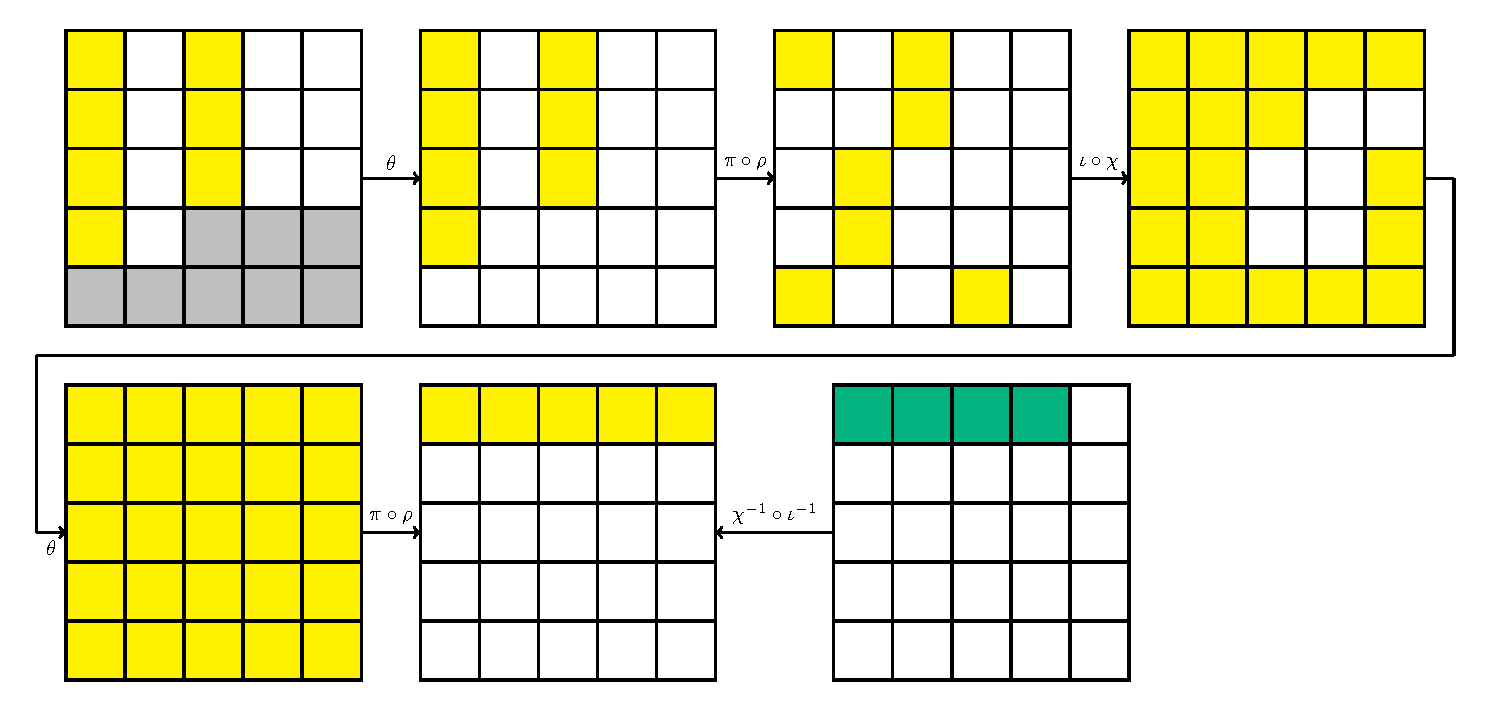
\includegraphics[scale=0.6]{3Rkeccak256.pdf}
    }
        \caption{Preimage Attack on $3$-round \KECCAK-$256$}
        \label{fig:3rkeccak256}
\end{figure}

To prevent the spread of $\theta$ in the first round we need to add constraints :
\begin{enumerate}
\item \[
        A[0,0] = A[0,1] \oplus A[0,2] \oplus A[0,3] \oplus \alpha_0
    \]
\item \[
        A[2,0] = A[2,1] \oplus A[2,2] \oplus \alpha_2
    \]
\end{enumerate}
where, $\alpha_0, \alpha_2$ are random constants.

Due to the above constraints, the state remains linear and the variables do not spread after application of $\theta$ step mapping as shown in the second state of the Figure~\ref{fig:3rkeccak256}. Further applying $\pi \circ \rho$ on the second state, permutes the positions of the lanes as well as rotations within the lane. Following this, $\iota \circ \chi$ step is applied to the third state to obtain the fourth state, which is a linear state. As explained in observation~\ref{ob5} since $\chi$ is a row-dependent operation and each row in the third state contains at most $2$ variables which are not adjacent therefore the resultant row after applying $\chi$ doesn't contain any quadratic variables.

Hence after applying $\iota \circ \chi \circ \pi \circ \rho \circ \theta $ i.e. one round on the initial state, the output state remains linear.

Moving on to the second round, the state is linear even after application of $\pi \circ \rho \circ \theta$, since these step mappings are linear and they don't introduce any non-linear terms. The input state (i.e. state $A$ as shown in Figure~\ref{fig:3rkeccak256}) to $\chi$ step of the second round is linear. Each row of state $A$ contains adjacent linear variables, therefore, we obtain non-linear terms in state $B$ after applying $\chi$ step. This is due to the fact that $\chi$ is a non-linear operation.

% On the other hand, for \KECCAK-$256$ we have $d = 256 = 64*4$ i.e. hash value of only $4$ lanes. To make it easier to invert the $\chi$ step we can assume any random value as the value of the 5th lane in the hash state. but this will add more conditions to satisfy those assumed 64 bits for the 5-th lane.
% We can directly apply $\iota^{-1}$ on the given hash and then we obtain $4$ hash lanes. Further, we can apply observation~\ref{ob3} to obtain $4$ linear equations on the bits input to $\chi$ for that row. By this, we obtain linear relations for the input state to the $\chi$ step.

Then we can apply the same technique as mentioned in section~\ref{3rkeccak512attack} for this structure also. If we observe then, each bit of the inverted hash state is a sum of $11$ bits (due to $\theta$ step) of the output of the second round. Since $\pi \circ \rho$ just permutate the positions of these bits and $\iota$ just adds a constant to the first lane, they do not increase the nonlinear terms, and thus we can ignore these step mappings in the last one and a half rounds. For $3$ rounds of \Keccak-$256$ the hash state comprises of 4 lanes. We can't directly apply $\chi^{-1} \circ \iota^{-1}$ on the hash state since we know only $4$ out of $5$ bits in row-$0$ of hash state. For this attack we can use observation~\ref{ob4} to set up equations such as $a_0 = b_0$ when $b_1 = 1$~\cite{guo2016linear}. Here $a_i,b_i$ denotes the input and output bit of $\chi$ respectively. 

Now, we aim to linearize $C[x][y][z]$ by guessing a few terms and then matching it with the bit obtained after applying $\chi^{-1}$ as explained above.

The state $C$ in Figure~\ref{fig:3rkeccak256}, can be expressed in terms of state $B$ :
\[
    C[x][y][z] = B[x][y][z] \oplus \oplus_{y' = 0}^{4} B[x-1][y'][z] \oplus \oplus_{y' = 0}^{4} B[x+1][y'][z-1]
\]

Open all the expressions and separate two terms $B[x][y][z]$ and $B[x-1][y][z]$ and rest 9 terms remain as it is.
So, \[ B[x][y][z] \oplus B[x-1][y][z] = (a \oplus c + b) \oplus d
    \]
Where,
\[
    a = A[x][y][z], b = A[x + 1][y][z], c = A[x + 2][y][z], d = A[x - 1][y][z]
\]
Guessing $b$ and other $9$ terms would make $C[x][y][z]$ linear. Hence, We linearize $C[x][y][z]$ by guessing these $10$ bits. We obtain $11 = 1 + 10$ linear equations and match $1$ bit of the hash value corresponding to $C[x][y][z]$. So, if we have $t$ variables in our state, then we can match $t/11$ bits of the hash.

For \Keccak-$256$, we started with $7$ lanes variable states in the initial state. After applying conditions to keep $\theta$ as constant we are left with $7 - 2 = 5$ lane variables. Hence $t = 5 \cdot 64 = 320$ variables.
Therefore, the number of matched bits of the hash are $t/11 = 320/11 = 29$, with this we have a complexity gain over brute-force of $2^{29}$.

Attack complexity $ = 2^{256 - 29} = 2^{227}$.

So the attack complexity for $3$ rounds of \KECCAK{}-$256$ is $2^{227}$.

\section{Preimage Attack on 3 rounds of \KECCAK-224}

In this section, we discuss a preimage attack for $3$ rounds of \KECCAK{}-$224$ where we try to keep the first $2$ rounds linear and then build a system of $128$ linear equations on $128$ variables from the $224$-bit hash.

\KECCAK{}-$224$ has hash length $d=224$, capacity $c=448$ and rate $r = 1152 = 18$ lanes. We start with the initial state as shown in Figure~\ref{fig:3rkeccak224} where the yellow lanes represent linear variables, blue lanes represent lanes containing all bits as $1$ and white lanes represent lanes containing all bits as $0$. To prevent the spread of linear variables by $\theta$ step we add the following constraints:

\begin{enumerate}
	\item \[
	A[0,0] = A[0,1] \oplus A[0,2] \oplus A[0, 3]
	\]
	\item \[
	A[2,0] = A[2,1] \oplus A[2,2] \oplus A[2,3]
	\]
\end{enumerate}

\begin{figure}[H]
	\resizebox{\linewidth}{!}{
	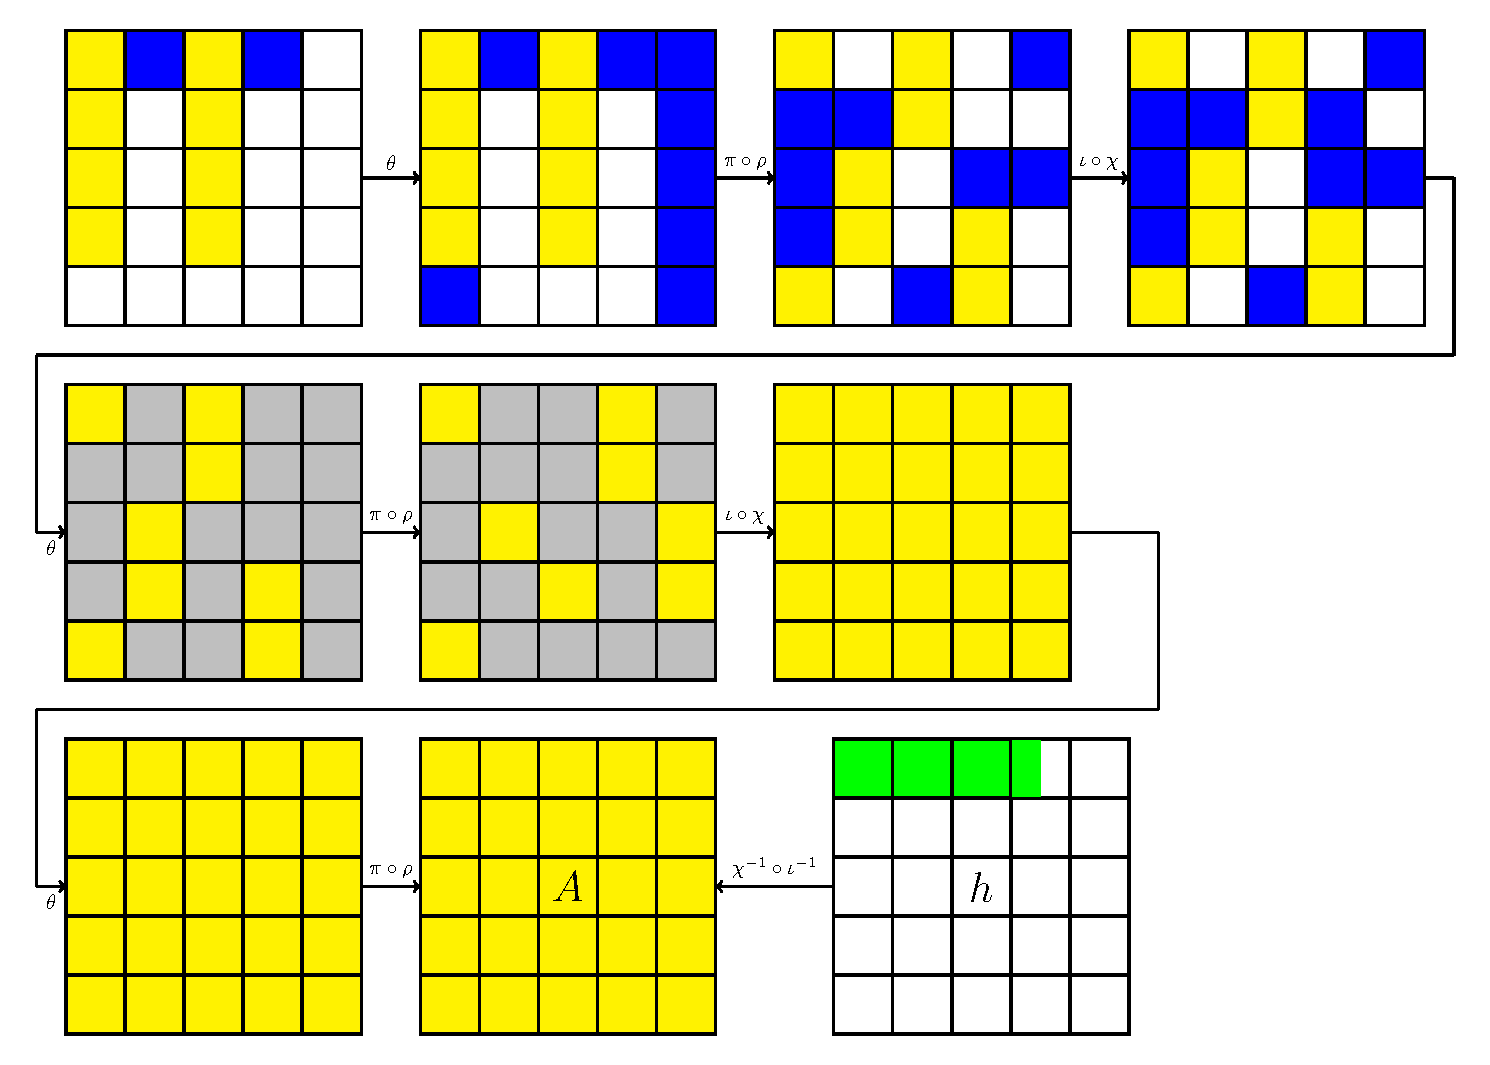
\includegraphics[scale=0.7]{3R,Keccak-224.pdf}
}
	\caption{Preimage Attack on 3-round \KECCAK-$224$}
	\label{fig:3rkeccak224}
\end{figure}

Due to the above constraints, after $\theta$ step the variables in the column $0$ and $2$ doesn't spread. Moreover, the parity of column-$1$ and column-$3$ is $1$ which causes the increase in the number of lanes containing all bits as $1$ after $\theta$ as shown in the second state of Figure~\ref{fig:3rkeccak224}. After applying $\pi \circ \rho$ on the second state, the position of lanes is permuted as shown in the third state. Further, on applying $\iota \circ \chi$ we obtain the fourth state, we observe that there is no increase in the number of linear terms in this state this is primarily due to the values of the rows input to $\chi$. With this, the first round is complete and the output state i.e. fourth state is still linear.

We now proceed with the second round, since there are $4$ columns in the fourth state with linear terms in Figure~\ref{fig:3rkeccak224}. These linear variables will spread after the $\theta$ step of second round, to prevent this we constraint the parity of these $4$ columns to be random constants. After applying the $\theta$ step we obtain the fifth state where the yellow lanes represent the linear variables and gray lanes represent constants. On the application of $\pi \circ \rho$ on the fifth state, the position of all lanes is permuted. Now after applying $\iota \circ \chi$ on the sixth state we observe that all the lanes in the seventh state contain linear terms, this is primarily due to atmost 2 linear terms in some rows of the state input to $\chi$ as explained in observation~\ref{ob5}. Due to this the complete row after applying $\chi$ contains linear terms. With this, the second round is complete and the output state i.e. seventh state where all lanes are linear as shown in~\ref{fig:3rkeccak224}.

Further, we start with the third round. After applying $\pi \circ \rho \circ \theta$ steps on the seventh state we obtain state $A$ which is linear as all these steps are linear mappings. For \Keccak{}-$224$, the hash state comprises of $3$ lanes and $32$ bits in the 4th lane as shown in green lanes in~\ref{fig:3rkeccak224}. We can't directly apply $\chi^{-1} \circ \iota^{-1}$ on the hash state since we don't have value of complete row. For this attack we can use observation~\ref{ob3} for the first $32$ slices of the hash state and obtain $4$ linear equations for each slice on the state $A$ i.e. input state to the $\chi$ step of third round. In the initial state, we have $8$ yellow lanes and after applying conditions for the first and second rounds of $\theta$ we are left with $8 - 2 - 4 = 2$ variable lanes. Therefore, the size of the linear structure is $2$ lanes = $128$ bits. All the bits in state $A$ are expressed in the form of these $128$ variables, we setup $128$ linear equations on $128$ variables from a $224$-bit hash value. We expect a complexity gain over bruteforce of $2^{128}$ and then can expect a correct preimage in $2^{224 - 128} = 2^{96}$ tries. The complexity of this attack is $O(2^{96})$.

\section{Preimage Attack on 4 rounds of \KECCAK-224}
    
In this section, we discuss a preimage attack for $4$ rounds of \KECCAK{}-$224$ where we try to keep the first $2$ rounds linear and then linearize the initial state of the $4$th round to be able to match some bits of the hash.

We start with the initial state as shown in Figure~\ref{fig:keccak224} where the yellow lanes represent linear variables, blue lanes represent lanes containing all bits as $1$ and white lanes represent lanes containing all bits as $0$. To prevent the spread of linear variables by $\theta$ step we add the following constraints:

\begin{figure}[H]
	\resizebox{\linewidth}{!}{
    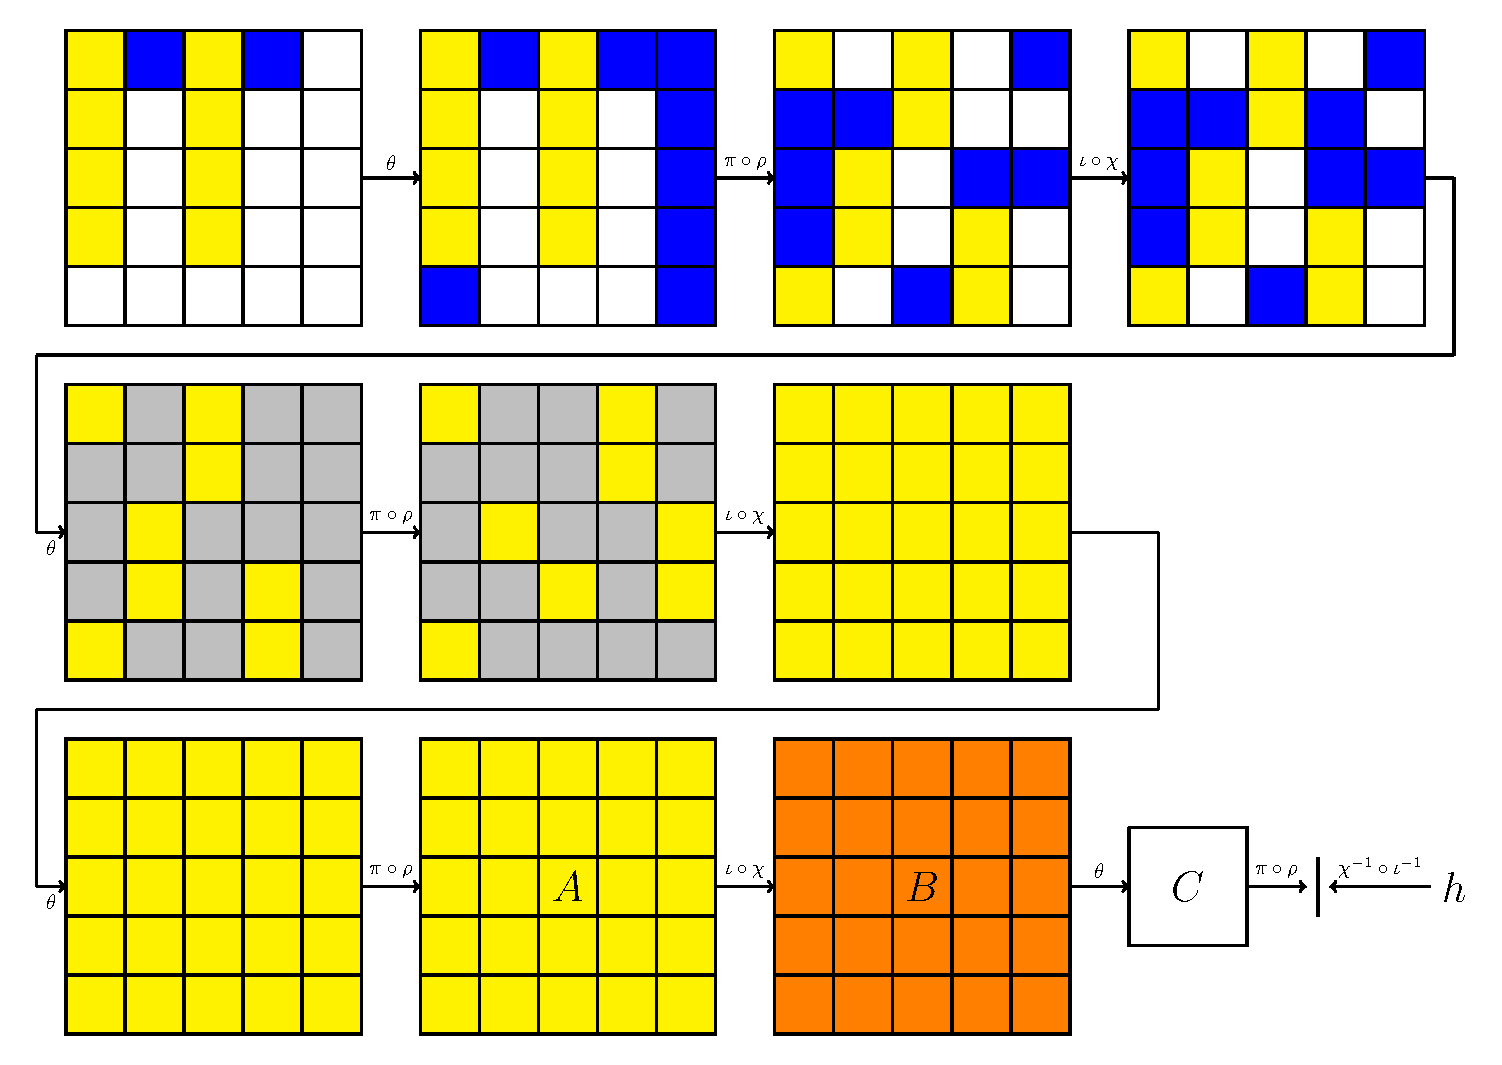
\includegraphics[scale=0.7]{4R,Keccak-224.pdf}
}
    \caption{Preimage Attack on 4-round \KECCAK-$224$}
    \label{fig:keccak224}
\end{figure}



\begin{enumerate}
    \item \[
        A[0,0] = A[0,1] \oplus A[0,2] \oplus A[0, 3]
    \]
\item \[
        A[2,0] = A[2,1] \oplus A[2,2] \oplus A[2,3]
    \]
\end{enumerate}

Due to the above constraints, after $\theta$ step the variables in the column $0$ and $2$ doesn't spread. Moreover, the parity of column-$1$ and column-$3$ is $1$ which causes the increase in the number of lanes containing all bits as $1$ after $\theta$ as shown in the second state of Figure~\ref{fig:keccak224}. After applying $\pi \circ \rho$ on the second state, the position of lanes is permuted as shown in the third state. Further on applying $\iota \circ \chi$ we obtain the fourth state, we observe that there is no increase in the number of linear terms. This is due to the values of the rows input to $\chi$ of first round. With this, the first round is complete and the output state i.e. fourth state is still linear.

We now proceed with the second round, since there are $4$ columns in the fourth state with linear terms of Figure~\ref{fig:keccak224}. These linear variables will spread after the $\theta$ step, to prevent this we constraint the parity of these $4$ columns to be random constants. After applying the $\theta$ step we obtain the fifth state where the yellow lanes represent the linear variables and gray lanes represent constants. On the application of $\pi \circ \rho$ on the fifth state, the position of all lanes is permuted. Now after applying $\iota \circ \chi$ on the sixth state we observe that almost all the lanes state in the seventh state contain linear terms, this is primarily due to 2 linear terms in few rows in the state input to $\chi$ as explained in observation~\ref{ob5}. Due to this the complete row after applying $\chi$ contains linear terms. With this, the second round is complete and the output state i.e. seventh state where all lanes are linear as shown in~\ref{fig:keccak224}.

Further, we start with the third round. After applying $\theta$ step on the seventh state the state remains linear as $\theta$ is a linear operation. After applying $\pi \circ \rho$ we obtain state $A$ which is linear as $\pi$ and $\rho$ steps are linear step mappings. In state $A$ each row contains linear variables, and since $\chi$ is a non-linear operation so if two adjacent bits are linear in a row then the output state will contain non-linear terms after applying $\chi$. So on applying step $\chi$ to state $A$, we obtain state $B$ where orange lanes represent non-linear as shown in ~\ref{fig:keccak224}.

If we carefully observe then the input to step $\chi$ of the third round is linear i.e. state $A$ and also that each bit of the input state of the $\chi$ step of the fourth round is a sum of $11$ bits (due to $\theta$ step) of the output state of the third round. Since $\pi \circ \rho$ just permutate the positions of these bits and $\iota$ just adds a constant to the first lane so they don't increase the nonlinear terms. Therefore, we ignore these step mappings in the last one and a half rounds.

For \Keccak{}-$224$ the hash state comprises of 3 lanes and 32 bits in the 4th lane. We can't directly apply $\chi^{-1} \circ \iota^{-1}$ on the hash state since we don't have value of complete row. For this attack we can use observation~\ref{ob4} to set up equations such as $a_0 = b_0$ when $b_1 = 1$~\cite{guo2016linear}. Here $a_i, \; b_i$ denotes the input and output bit of $\chi$ respectively.

The state $C$ in Figure~\ref{fig:keccak224}, can be expressed in terms of state $B$ :
\[
C[x][y][z] = B[x][y][z] \oplus \oplus_{y' = 0}^{4} B[x-1][y'][z] \oplus \oplus_{y' = 0}^{4} B[x+1][y'][z-1]
\]

Open all the expressions and separate two terms $B[x][y][z]$ and $B[x-1][y][z]$ and rest 9 terms remain as it is.
So, \[ B[x][y][z] \oplus B[x-1][y][z] = (a \oplus c + b) \oplus d
\]
Where,
\[
a = A[x][y][z], b = A[x + 1][y][z], c = A[x + 2][y][z], d = A[x - 1][y][z]
\]
Guessing $b$ and other 9 terms would make $C[x][y][z]$ linear. Hence, We linearize $C[x][y][z]$ by guessing these 10 bits. We obtain 11 = 1 + 10 linear equations and match 1 bit of the hash value corresponding to $C[x][y][z]$. So, if we have $t$ variables in our state, then we can match $t/11$ bits of the hash.

For \Keccak-$224$, we started with $8$ variable lanes in the initial state. After applying conditions to keep $\theta$ as constant in the first and the second round we are left with $8 - 2 - 4 = 2$ variable lane. Hence the number of variables $t = 2\cdot 64 = 128$. From these variables we can match atmost $t/11 = 128/11 = 11$ bits. 
With this, we have a complexity gain over the brute-force of $2^{11}$.

Attack complexity $ = 2^{224 - 11} = 2^{213}$.